\chapter{Rezultati} % Main chapter title
\label{Chapter6}

Za svaki od tri prethodno opisana metoda binarne klasifikacije trenirano je po 399 modela na celom trening skupu koji su kasnije ujedinjeni u 3 prediktora za predviđanje funkcije proteina. Pored toga, implementiran je još jedan jednostovaniji klasifikator koji je poslužio kao osnovna metoda za poređenje rezultata. U pitanju je naivni klasifikator koji svakom čvoru dodeljuje vrednost koja odgovara njegovoj frekvenciji pojavljivanja u trening skupu i tako formirani graf pridružuje svakom test primeru \cite{doktJK}. 

Naivni klasifikator je testiran na istom test skupu kao i 3 prediktora, a rezultat je prikazan na slici \ref{fig:f1scores}. Prilikom svakog testiranja računata je prosečna vrednost $f_1$ mere i to na nivou pojedinačnih organizama, kao i na nivou celog skupa. Sa slike se može videti da je svaki od tri prediktora bolji od naivnog klasifikatora. Pored toga, metod potpornih vektora daje najbolje rezultate kako za pojedinačne organizme, tako i za ceo skup.


\begin{figure}[h]
	\centering
	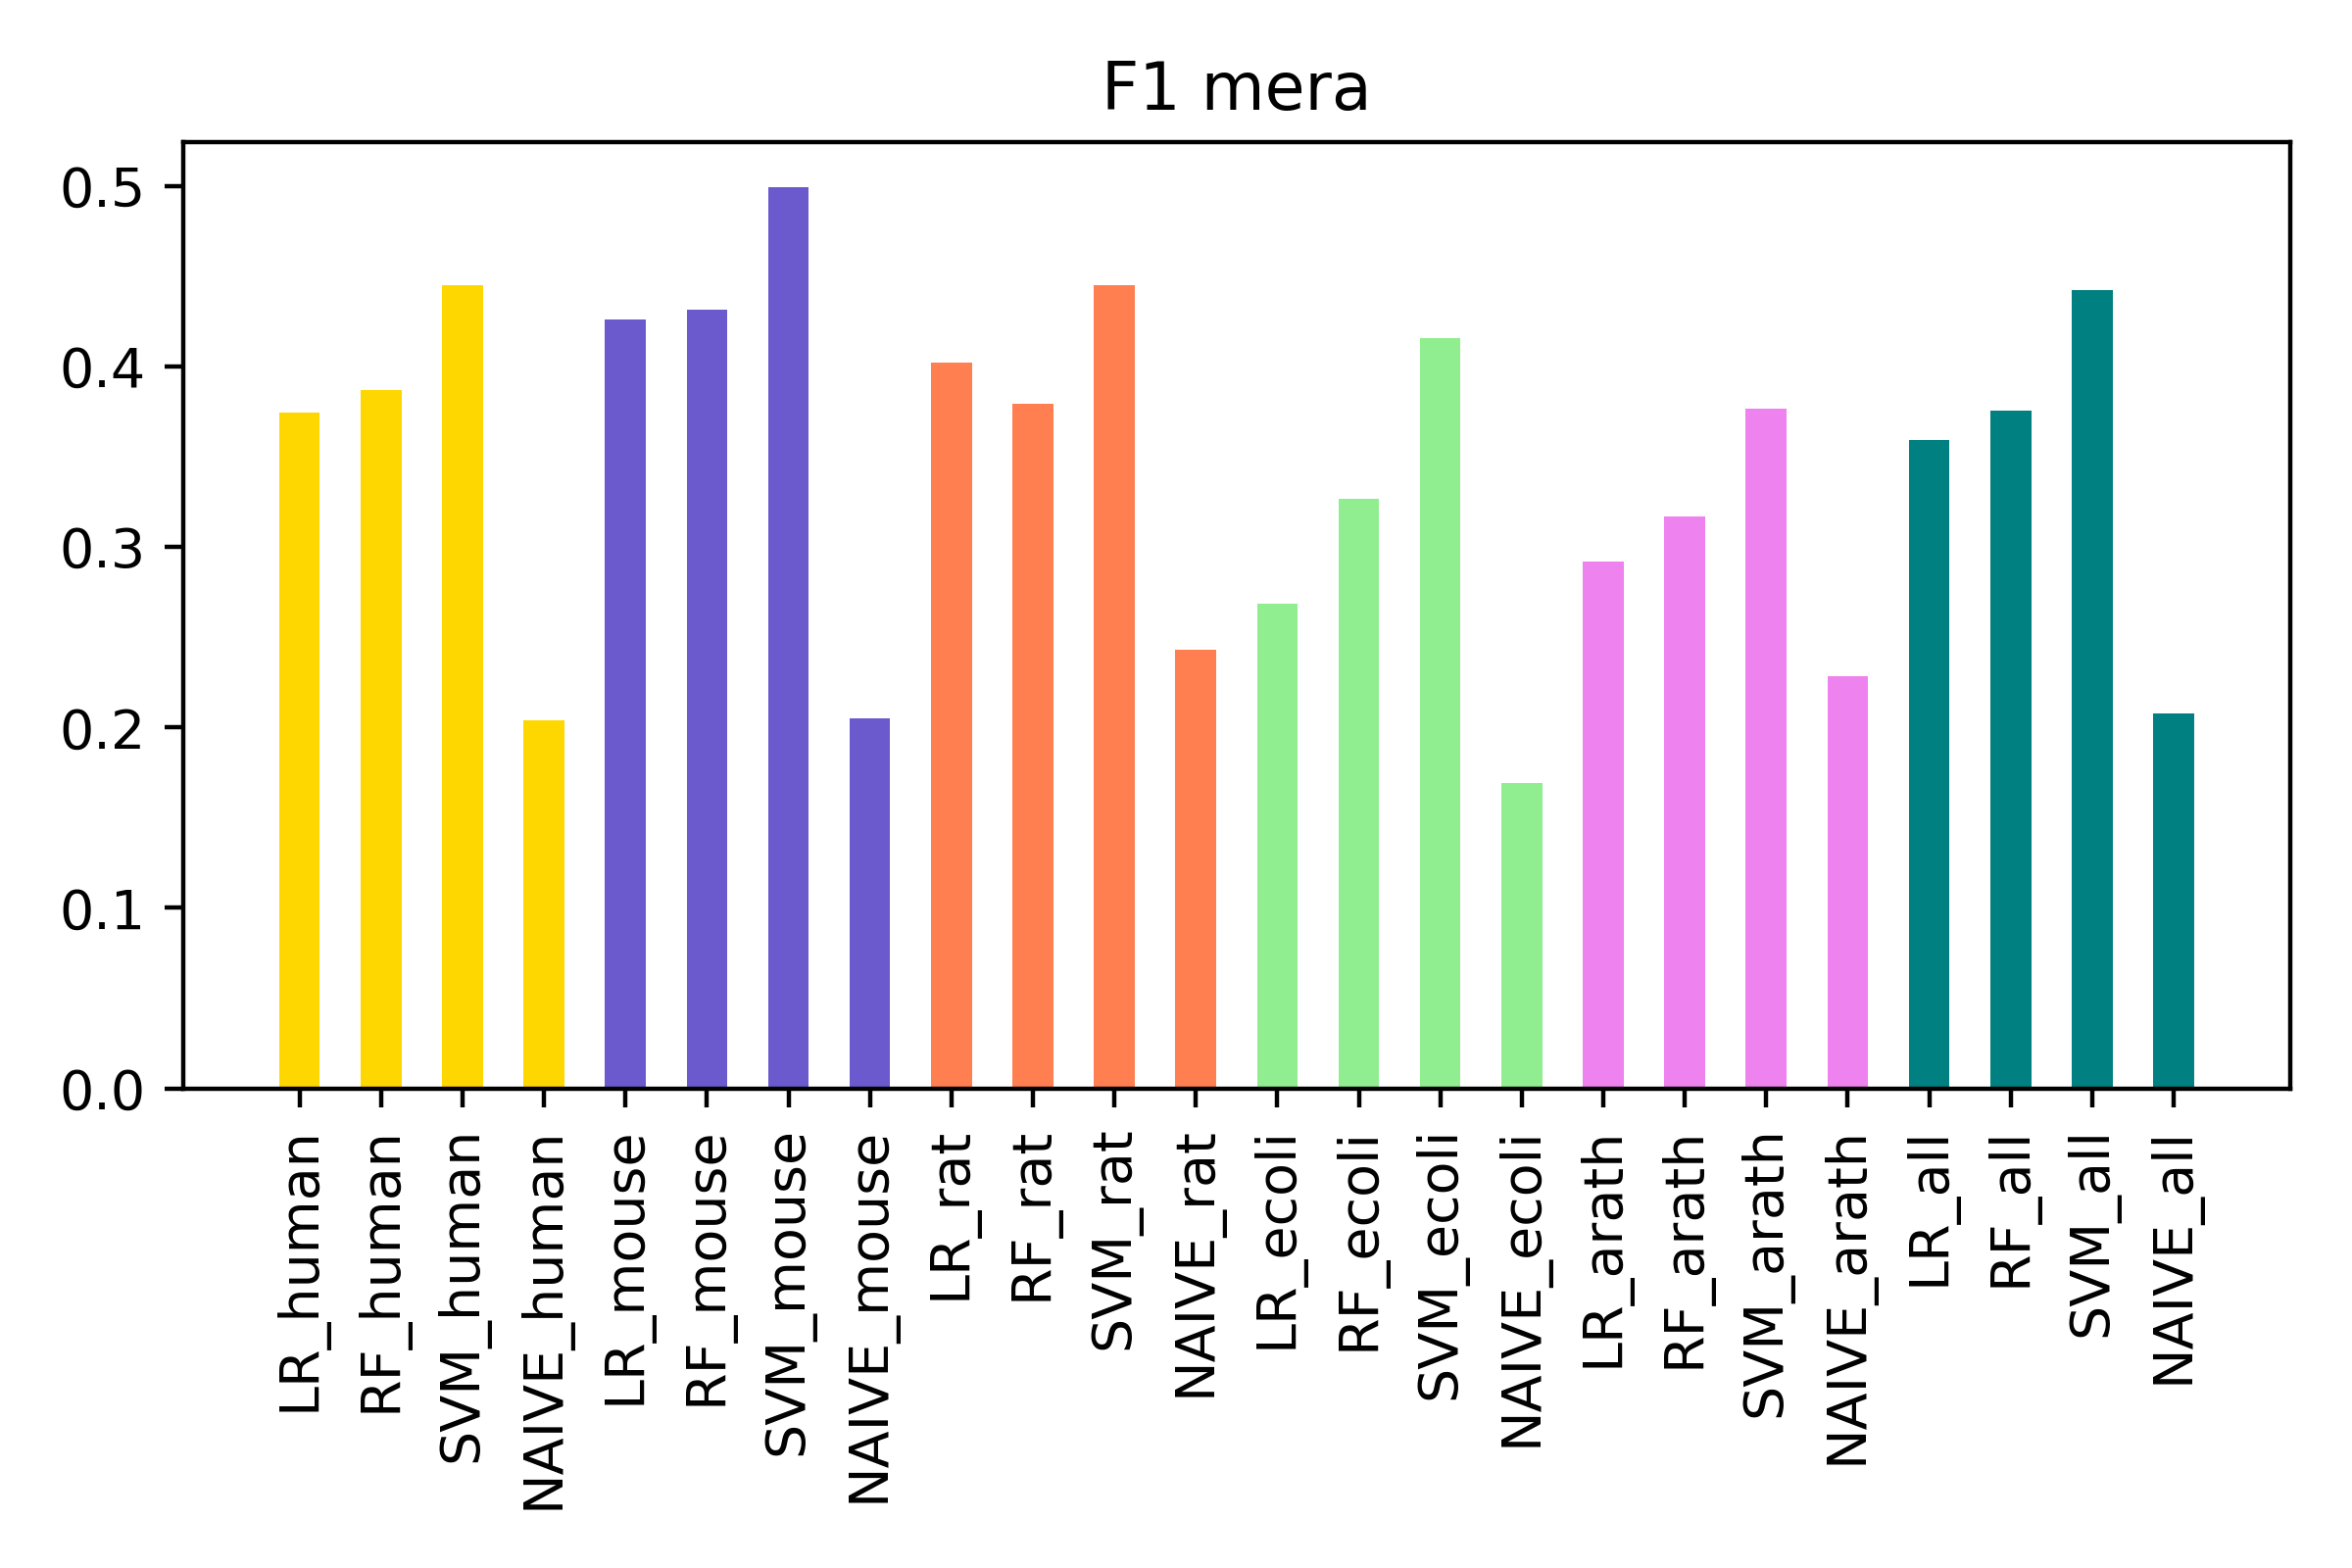
\includegraphics[width=\textwidth]{Figures/f1_scores.png}
	\caption{Poređenje performansi prediktora i naivnog klasifikatora. Rezultati jednog organizma prikazani su istom bojom.}
	\label{fig:f1scores}
\end{figure}


U tabelama \ref{tab: rfF1}, \ref{tab: lrF1} i \ref{tab: svmF1} prikazane su $f_1$ mere za 20 pojedinačnih klasifikatora za svaku upotrebljenu metodu binarne klasifikacije. Pored toga, prikazan je i broj pojavljivanja u trening skupu za svaku funkciju, kao i udeo broja pojavljivanja funkcije u celom trening skupu. Vrednosti za sve klasifikatore prikazane su na adresi \url{http://poincare.matf.bg.ac.rs/~anja_bukurov/master}.


\begin{table}[h]
	\centering
	\begin{tabular}{|c|c|c|c|}
		\hline
		Funkcija & f1-mera & Broj pojavljivanja u skupu & Procenat pojavljivanja u skupu \\		\hline
		GO:0005525 & 0.3 & 290 & 1.4\% \\
		\hline
		GO:0008134 & 0.11 & 861 & 4.1\% \\
		\hline
		GO:0019899 & 0.11 & 2381 & 11.4\% \\
		\hline
		GO:0044325 & 0.13 & 144 & 0.7\% \\
		\hline
		GO:0003723 & 0.12 & 1899 & 9.1\% \\
		\hline
		GO:0016787 & 0.25 & 3202 & 15.3\% \\
		\hline
		GO:0019900 & 0.12 & 5268 & 20.8\% \\
		\hline
		GO:0019888 & 0.13 & 71 & 0.3\% \\
		\hline
		GO:0004722 & 0.45 & 123 & 0.6\% \\
		\hline
		GO:0004867 & 0.18 & 105 & 0.5\% \\
		\hline
		GO:0005496 & 0.11 & 71 & 0.3\% \\
		\hline
		GO:0016829 & 0.12 & 316 & 1.5\% \\
		\hline
		GO:0046872 & 0.12 & 1824 & 8.7\% \\
		\hline
		GO:0016758 & 0.11 & 172 & 0.8\% \\
		\hline
		GO:0003729 & 0.13 & 5611 & 21.5\% \\
		\hline
		GO:0004930 & 0.12 & 312 & 1.5\% \\
		\hline
		GO:0030594 & 0.42 & 86 & 0.4\% \\
		\hline
		GO:0004497 & 0.16 & 5710 & 21.7\% \\
		\hline
		GO:0030246 & 0.18 & 180 & 0.9\% \\
		\hline
		GO:0031406 & 0.12 & 5730 & 21.7\% \\
		\hline
	\end{tabular}
	\caption{Prikaz f1-mere za pojedina\v cne klasifikatore metode slučajne šume}
	\label{tab: rfF1}
\end{table}

\begin{table}[h]
	\centering
	\begin{tabular}{|c|c|c|c|}
		\hline
		Funkcija & f1-mera & Broj pojavljivanja u skupu & Procenat pojavljivanja u skupu \\		\hline
		GO:0005525 & 0.46 & 290 & 1.4\% \\
		\hline
		GO:0005524 & 0.2 & 671 & 3.2\% \\
		\hline
		GO:0051117 & 0.11 & 101 & 0.5\% \\
		\hline
		GO:0008134 & 0.26 & 861 & 4.1\% \\
		\hline
		GO:0019899 & 0.31 & 2381 & 11.4\% \\
		\hline
		GO:0019904 & 0.15 & 681 & 3.3\% \\
		\hline
		GO:0044877 & 0.16 & 985 & 4.7\% \\
		\hline
		GO:0003714 & 0.16 & 292 & 1.4\% \\
		\hline
		GO:0046982 & 0.16 & 663 & 3.2\% \\
		\hline
		GO:0044325 & 0.28 & 144 & 0.7\% \\
		\hline
		GO:0003723 & 0.39 & 1899 & 9.1\% \\
		\hline
		GO:0031625 & 0.15 & 303 & 1.5\% \\
		\hline
		GO:0003779 & 0.28 & 402 & 1.9\% \\
		\hline
		GO:0030234 & 0.27 & 1047 & 5.0\% \\
		\hline
		GO:0019901 & 0.18 & 668 & 3.2\% \\
		\hline
		GO:0042803 & 0.15 & 1218 & 5.8\% \\
		\hline
		GO:0042802 & 0.25 & 2480 & 11.9\% \\
		\hline
		GO:0005102 & 0.3 & 1423 & 6.8\% \\
		\hline
		GO:0016787 & 0.49 & 3202 & 15.3\% \\
		\hline
		GO:0004222 & 0.46 & 128 & 0.6\% \\
		\hline
	\end{tabular}
	\caption{Prikaz f1-mere za pojedina\v cne klasifikatore metode logistička regresija}
	\label{tab: lrF1}
\end{table}

\begin{table}[h]
	\centering
	\begin{tabular}{|c|c|c|c|}
		\hline
		Funkcija & f1-mera & Broj pojavljivanja u skupu & Procenat pojavljivanja u skupu \\		\hline
		GO:0005525 & 0.36 & 290 & 1.4\% \\
		\hline
		GO:0005524 & 0.15 & 671 & 3.2\% \\
		\hline
		GO:0008134 & 0.27 & 861 & 4.1\% \\
		\hline
		GO:0019899 & 0.19 & 2381 & 11.4\% \\
		\hline
		GO:0044877 & 0.11 & 985 & 4.7\% \\
		\hline
		GO:0003714 & 0.15 & 292 & 1.4\% \\
		\hline
		GO:0046982 & 0.16 & 663 & 3.2\% \\
		\hline
		GO:0003723 & 0.33 & 1899 & 9.1\% \\
		\hline
		GO:0003779 & 0.24 & 402 & 1.9\% \\
		\hline
		GO:0030234 & 0.18 & 1047 & 5.0\% \\
		\hline
		GO:0019901 & 0.14 & 668 & 3.2\% \\
		\hline
		GO:0042802 & 0.11 & 2480 & 11.9\% \\
		\hline
		GO:0005102 & 0.15 & 1423 & 6.8\% \\
		\hline
		GO:0016787 & 0.43 & 3202 & 15.3\% \\
		\hline
		GO:0004222 & 0.24 & 128 & 0.6\% \\
		\hline
		GO:0019888 & 0.21 & 71 & 0.3\% \\
		\hline
		GO:0004722 & 0.43 & 123 & 0.6\% \\
		\hline
		GO:0004867 & 0.18 & 105 & 0.5\% \\
		\hline
		GO:0030145 & 0.11 & 162 & 0.8\% \\
		\hline
		GO:0051287 & 0.2 & 123 & 0.6\% \\
		\hline
	\end{tabular}
	\caption{Prikaz f1-mere za pojedina\v cne klasifikatore metode potpornih vektora}
	\label{tab: svmF1}
\end{table}


Iako su se trenirani prediktori pokazali bolje od naivnog klasifikatora, nemaju približnu moć predviđanja u poređenju sa aktivnim rezultatima prikazanim na poslednjem CAFA takmičenju, najrelevantnijem takmičenju u ovoj oblasti. Planovi za unapređenje prediktora uključuju treniranje posebnih modela za svaki od organizama na skupu proteina koji potiču isključivo iz odabranog organizma, zatim povećanje trening skupa i korišćenje raznovrsnijih  metoda binarne klasifikacije.

